\newthought{\textbf{Siti Hajar Al Zahra - 2020903430049 - TRKJ 3B}}

\newday{\textbf{1 - 2 Desember 2022} Instalasi dan Konfigurasi Apache Hadoop}
\begin{enumerate}
\item Kendala dan Solusi
\newline pada praktikum instalasi apache hadoop tidak terdapat kendala 
% jelaskan kendala dan penyebab yang dialami saat mengikuti praktikum serta solusi atau langkah-langkah yang telah dilakukan

\item Kesimpulan
\newline berhasil melakukan instalasi dan konfigurasi hadoop.
% berikan kesimpulan dari praktikum yang telah dikerjkan
\begin{figure}[!ht]
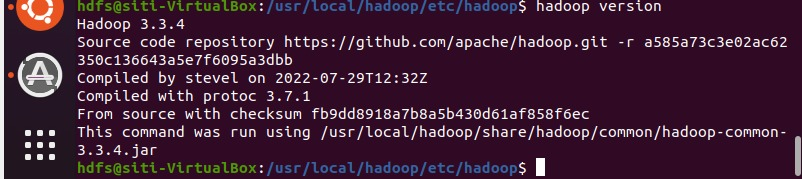
\includegraphics[width=\textwidth]{SitiHajarAlZahara/1}
\caption{hasil instalasi java}
\label{gam:Hasil}
\end{figure}

\begin{figure}[!ht]
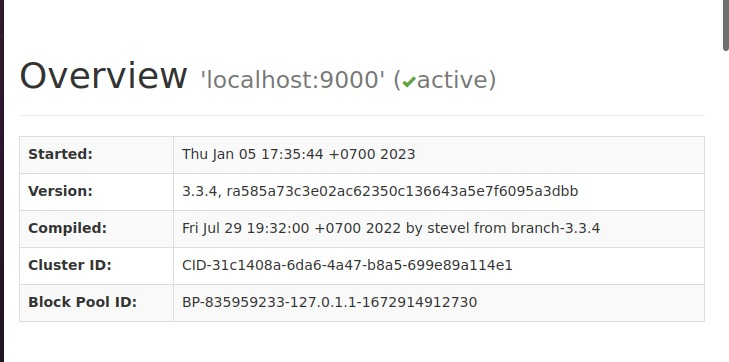
\includegraphics[width=\textwidth]{SitiHajarAlZahara/2}
\caption{hasil konfigurasi apache hadoop}
\label{gam:Hasil}
\end{figure}

\begin{figure}[!ht]
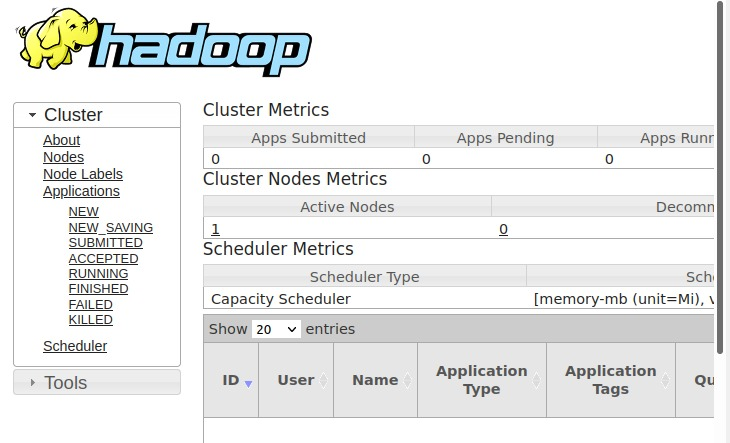
\includegraphics[width=\textwidth]{SitiHajarAlZahara/3}
\caption{hasil konfigurasi apache hadoop}
\label{gam:Hasil}
\end{figure}


\end{enumerate}

\newday{\textbf{8 - 9 Desember 2022} WordCount bawaan Hadoop}
\begin{enumerate}
\item Kendala dan Solusi
\newline pada praktikum wordcount ini pratikan tidak terdapat kendala 
% jelaskan kendala dan penyebab yang dialami saat mengikuti praktikum serta solusi atau langkah-langkah yang telah dilakukan

\item Kesimpulan
\newline berhasil melakukan konfigurasi WordCount Hadoop.
% berikan kesimpulan dari praktikum yang telah dikerjkan
\begin{figure}[!ht]
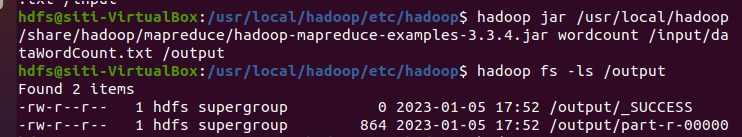
\includegraphics[width=\textwidth]{SitiHajarAlZahara/4}
\caption{ folder input di HDFS}
\label{gam:Hasil}
\end{figure}

\begin{figure}[!ht]
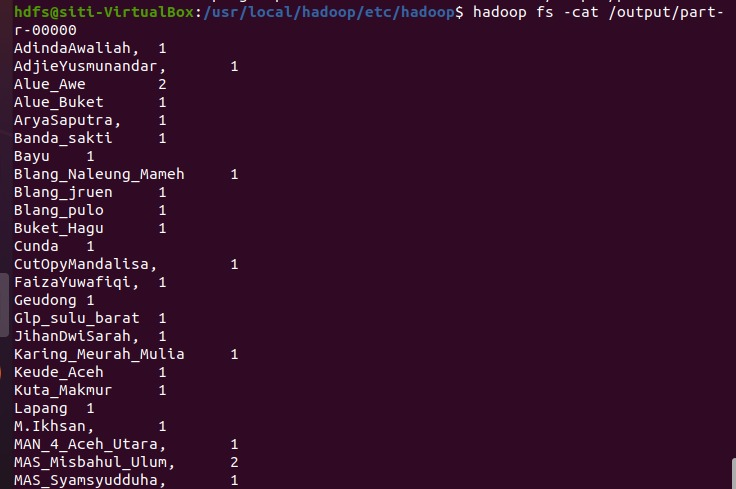
\includegraphics[width=\textwidth]{SitiHajarAlZahara/5}
\caption{hasil nama dan data wordcount}
\label{gam:Hasil}
\end{figure}

\begin{figure}[!ht]
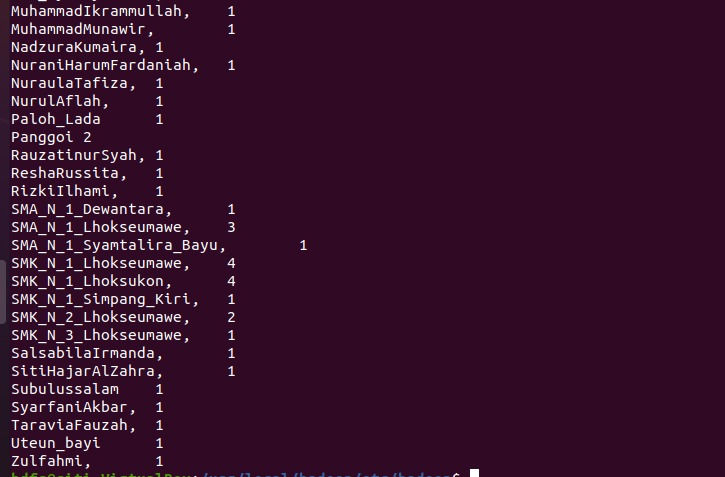
\includegraphics[width=\textwidth]{SitiHajarAlZahara/6}
\caption{hasil nama dan data wordcount}
\label{gam:Hasil}
\end{figure}
\end{enumerate}

\newday{\textbf{ 9 Desember 2022} program WordCount dengan java }
\begin{enumerate}
\item Kendala dan Solusi
\newline pada praktikum ini praktikan tidak terdapat kendala 
% jelaskan kendala dan penyebab yang dialami saat mengikuti praktikum serta solusi atau langkah-langkah yang telah dilakukan

\item Kesimpulan
\newline berhasil melakukan program WordCount dengan java.
% berikan kesimpulan dari praktikum yang telah dikerjkan
\begin{figure}[!ht]
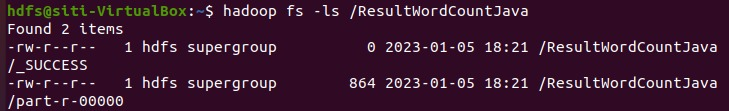
\includegraphics[width=\textwidth]{SitiHajarAlZahara/7}
\caption{hasil wordcount java}
\label{gam:Hasil}
\end{figure}

\begin{figure}[!ht]
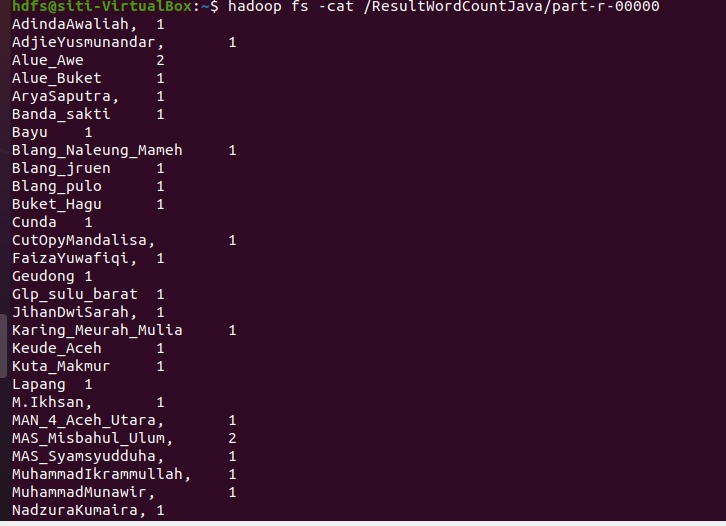
\includegraphics[width=\textwidth]{SitiHajarAlZahara/8}
\caption{hasil wordcount java}
\label{gam:Hasil}
\end{figure}

\begin{figure}[!ht]
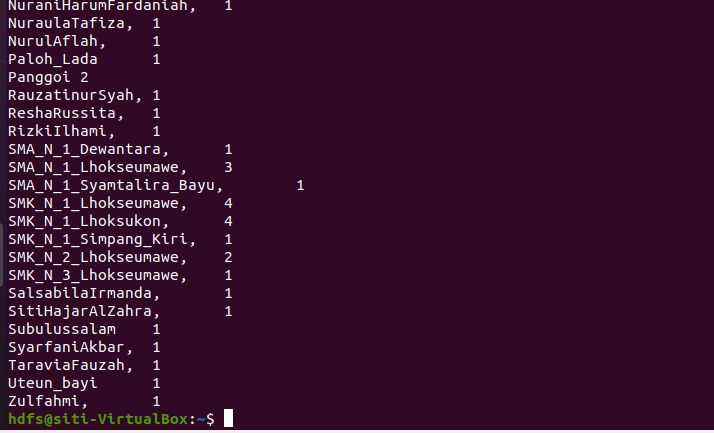
\includegraphics[width=\textwidth]{SitiHajarAlZahara/9}
\caption{hasil wordcount java}
\label{gam:Hasil}
\end{figure}
\end{enumerate}

\newday{\textbf{ 15 Desember 2022} Instalasi Apacahe PySpark }
\begin{enumerate}
\item Kendala dan Solusi
\newline pada praktikum instalasi Apache PySpar ini praktikan tidak terdapat kendala 
% jelaskan kendala dan penyebab yang dialami saat mengikuti praktikum serta solusi atau langkah-langkah yang telah dilakukan

\item Kesimpulan
\newline berhasil melakukan instalasi PySpark dan tidak terdapat kendala apapun.
% berikan kesimpulan dari praktikum yang telah dikerjkan
\begin{figure}[!ht]
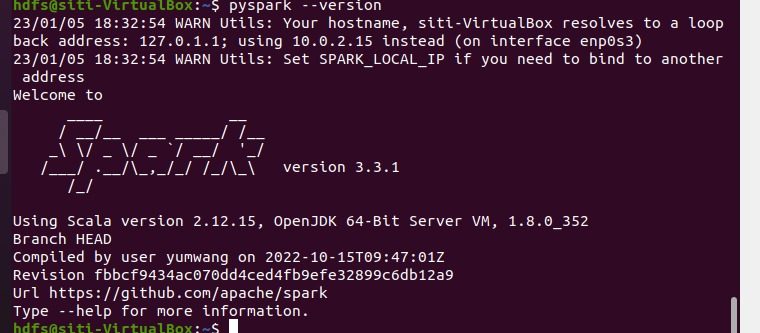
\includegraphics[width=\textwidth]{SitiHajarAlZahara/10}
\caption{hasil instalali Apache PySpark}
\label{gam:Hasil}
\end{figure}
\end{enumerate}
